% Figure 2c -- attribution logic: every captured request is labelled on four axes and joined to
% page-level facts. Final printed size: 116 mm x 56 mm (Figure 2, row 2, left).
% Sources: ../../crawl/vendor_endpoints.json (endpoint map; shopify_web_pixels_urls patterns),
% ../../crawl/cmp_signatures.json (CMP, declared blocklist, Shopify consent read-out),
% ../../notes/mechanism.md section 6 (what the crawler records).
% Origin encoding matches Fig 1a and Fig 3c: hatch = sandbox, solid light grey = main thread.
\documentclass[tikz,border=2pt]{standalone}
% schematic_style.tex -- shared style for every TikZ schematic panel (Fig 1a, 2a-2d).
% Binding source: ../../FIGURE_PLAN.md (style guide). Change colours here only.
% one sans face in BOTH engines (matplotlib panels use Arial too); Courier New for code (review: typography)
\usepackage{fontspec}\setmainfont{Arial}\setsansfont{Arial}\setmonofont{Courier New}
\renewcommand{\familydefault}{\sfdefault}
\usepackage{xcolor}
\usetikzlibrary{arrows.meta,calc,patterns.meta,shapes.geometric,positioning}

% ---- fixed vendor colours (FIGURE_PLAN.md, validated categorical order) ----
\definecolor{vGoogle}{HTML}{2A78D6}
\definecolor{vTikTok}{HTML}{EB6834}
\definecolor{vMeta}{HTML}{1BAF7A}
\definecolor{vPinterest}{HTML}{EDA100}
\definecolor{vSnap}{HTML}{E87BA4}
\definecolor{vMicrosoft}{HTML}{008300}
\definecolor{vOther}{HTML}{4A3AA7}
% ---- neutrals, arms (shape + grey, never hue), accent ----
\definecolor{ink}{HTML}{0B0B0B}      % text; Default arm
\definecolor{greyD}{HTML}{52514E}    % box outlines; Decline + Repeat arms
\definecolor{greyM}{HTML}{8A8984}    % sandbox hatch; GPC arm; secondary text
\definecolor{greyL}{HTML}{DEDDD9}    % main-thread origin (solid light grey)
\definecolor{greyXL}{HTML}{F3F2EF}   % faint container fill
\definecolor{accent}{HTML}{D03B3B}   % ONLY meaning: consent failed / blind spot
\colorlet{tbdgrey}{greyM}

% ---- sizes: 7 pt body, 10 pt bold panel letter ----
\newcommand{\fsBody}{\fontsize{7}{8.2}\selectfont}
\newcommand{\fsLetter}{\fontsize{10}{12}\selectfont\bfseries}
\newcommand{\fsTitle}{\fontsize{8}{9.6}\selectfont\bfseries}   % panel titles: 8 pt bold, as in the matplotlib panels (review FIG-20)

\tikzset{
  x=1mm, y=1mm,
  every picture/.style={line width=0.4pt},
  every node/.style={font=\fsBody, text=ink, inner sep=0.6mm},
  % arrows
  arr/.style={-{Stealth[length=1.5mm,width=1.1mm]}, draw=ink, line width=0.45pt},
  arrg/.style={-{Stealth[length=1.5mm,width=1.1mm]}, draw=greyD, line width=0.45pt},
  % boxes
  box/.style={draw=greyD, fill=white, rounded corners=0.7mm, line width=0.4pt},
  mainthread/.style={fill=greyL},
  sandbox/.style={pattern={Lines[angle=45,distance=1.25pt,line width=0.35pt]}, pattern color=greyM},
  % text helpers
  lbl/.style={align=left, anchor=north west, inner sep=0pt},
  lblc/.style={align=center, inner sep=0pt},
  note/.style={align=left, inner sep=0pt, text=greyD},
  panelletter/.style={font=\fsLetter, anchor=north west, inner sep=0pt},
  % arm markers (FIGURE_PLAN: Default filled circle #0b0b0b; Decline open square #52514e;
  % GPC filled triangle #8a8984; Repeat/validation open diamond #52514e)
  mDefault/.style={circle, fill=ink, draw=ink, inner sep=0pt, minimum size=2.1mm},
  mDecline/.style={rectangle, fill=white, draw=greyD, line width=0.7pt, inner sep=0pt, minimum size=1.85mm},
  mGPC/.style={regular polygon, regular polygon sides=3, fill=greyM, draw=greyM, inner sep=0pt, minimum size=2.7mm},
  mRepeat/.style={diamond, fill=white, draw=greyD, line width=0.7pt, inner sep=0pt, minimum size=2.4mm},
}

% vendor chip: \chip{vTikTok}  (small filled square; identity is always also named in text)
\newcommand{\chip}[1]{\tikz[baseline=-0.1mm]\fill[#1] (0,0) rectangle (1.7mm,1.7mm);}
% origin swatches for legends, same encoding as the data figures (3c)
\newcommand{\swMain}{\tikz[baseline=-0.1mm]\draw[greyD,fill=greyL,line width=0.3pt] (0,0) rectangle (3.2mm,1.9mm);}
\newcommand{\swSand}{\tikz[baseline=-0.1mm]\draw[greyD,line width=0.3pt,pattern={Lines[angle=45,distance=1.25pt,line width=0.35pt]},pattern color=greyM] (0,0) rectangle (3.2mm,1.9mm);}
% inline arm markers for text
\newcommand{\mkDefault}{\tikz[baseline=-0.75mm]\node[mDefault]{};}
\newcommand{\mkDecline}{\tikz[baseline=-0.75mm]\node[mDecline]{};}
\newcommand{\mkGPC}{\tikz[baseline=-0.95mm]\node[mGPC]{};}
\newcommand{\mkRepeat}{\tikz[baseline=-0.75mm]\node[mRepeat]{};}
\newcommand{\blindstar}{\tikz[baseline=-0.35mm]\node[star,star points=5,star point ratio=2.3,fill=accent,inner sep=0pt,minimum size=2.3mm]{};}

% Exact final size: standalone adds a 2pt border on every side, so the drawn
% bounding box is (W - 4pt) x (H - 4pt) and the PDF is exactly W x H.
\newcommand{\panelsize}[2]{\path[use as bounding box] (0,0) rectangle ($(#1,#2)-(4pt,4pt)$);}
\newcommand{\panelletter}[2]{\node[panelletter] at ($(0,#2)-(0,4pt)$) {#1};}

\begin{document}
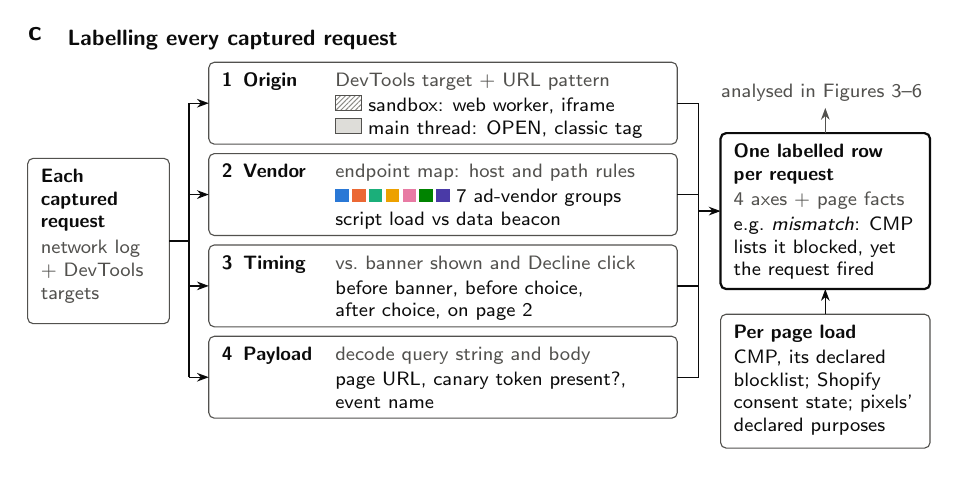
\begin{tikzpicture}
\def\W{116}\def\H{56}
\panelsize{\W}{\H}
\panelletter{c}{\H}
\node[lbl,font=\fsTitle] at (5,54.3) {{Labelling every captured request}};

% ---------------------------------------------------------------- input
\draw[box] (0,17) rectangle (18,38);
\node[lbl] at (1.6,36.7) {\textbf{Each}\\ \textbf{captured}\\ \textbf{request}\\[0.4mm] {\color{greyD}network log}\\ {\color{greyD}+ DevTools}\\ {\color{greyD}targets}};

% ---------------------------------------------------------------- four axes
% \axis{y-top}{number}{name}{how}{labels}
\newcommand{\axisbox}[5]{%
  \draw[box] (23,#1-10.4) rectangle (82.5,#1);
  \node[lbl] at (24.6,#1-1.3) {\textbf{#2\enspace#3}};
  \node[lbl] at (39,#1-1.3) {#4\\[0.3mm] #5};
  \coordinate (in#2) at (23,#1-5.2);
  \coordinate (out#2) at (82.5,#1-5.2);}
\axisbox{50.2}{1}{Origin}{{\color{greyD}DevTools target + URL pattern}}%
  {\swSand\ sandbox: web worker, iframe\\ \swMain\ main thread: OPEN, classic tag}
\axisbox{38.6}{2}{Vendor}{{\color{greyD}endpoint map: host and path rules}}%
  {\chip{vGoogle}\,\chip{vTikTok}\,\chip{vMeta}\,\chip{vPinterest}\,\chip{vSnap}\,\chip{vMicrosoft}\,\chip{vOther}\ 7 ad-vendor groups\\ script load vs data beacon}
\axisbox{27.0}{3}{Timing}{{\color{greyD}vs.\ banner shown and Decline click}}%
  {before banner, before choice,\\ after choice, on page 2}
\axisbox{15.4}{4}{Payload}{{\color{greyD}decode query string and body}}%
  {page URL, canary token present?,\\ event name}

% input -> axes (bus)
\draw[ink, line width=0.45pt] (18,27.5) -- (20.5,27.5);
\draw[ink, line width=0.45pt] (20.5,0 |- in4) -- (20.5,0 |- in1);
\foreach \i in {1,...,4} \draw[arr] (20.5,0 |- in\i) -- (in\i);

% ---------------------------------------------------------------- page-level facts + output
\draw[box] (88,1.2) rectangle (114.6,18.2);
\node[lbl] at (89.6,16.9) {\textbf{Per page load}\\[0.3mm] CMP, its declared\\ blocklist; Shopify\\ consent state; pixels'\\ declared purposes};

\draw[box, draw=ink, line width=0.8pt] (88,21.4) rectangle (114.6,41.2);
\node[lbl] at (89.6,39.9) {\textbf{One labelled row}\\ \textbf{per request}\\[0.3mm] {\color{greyD}4 axes + page facts}};
\node[lbl] at (89.6,30.6) {e.g.\ \emph{mismatch}: CMP\\ lists it blocked, yet\\ the request fired};

% axes -> output (bus)
\foreach \i in {1,...,4} \draw[ink, line width=0.45pt] (out\i) -- (85.2,0 |- out\i);
\draw[ink, line width=0.45pt] (85.2,0 |- out4) -- (85.2,0 |- out1);
\draw[arr] (85.2,31.3) -- (88,31.3);
\draw[arr] (101.3,18.2) -- (101.3,21.4);

\node[note, anchor=south west] at (88,45.2) {analysed in Figures 3--6};
\draw[arrg] (101.3,41.2) -- (101.3,44.4);
\end{tikzpicture}
\end{document}
